\chapter{Etat de l'Art}

%%%%%%%%%%%%%%%%%%%%%%%%%%%%%%%%%%%%%%%%%%%%%%%%%%%%%%%%%%%%%%%%%%%%%%%%%%%%%%%
\section{Présentation de l'ESP}
    \textbf{Aperçu}

    \begin{figure}[H]
        \centering
        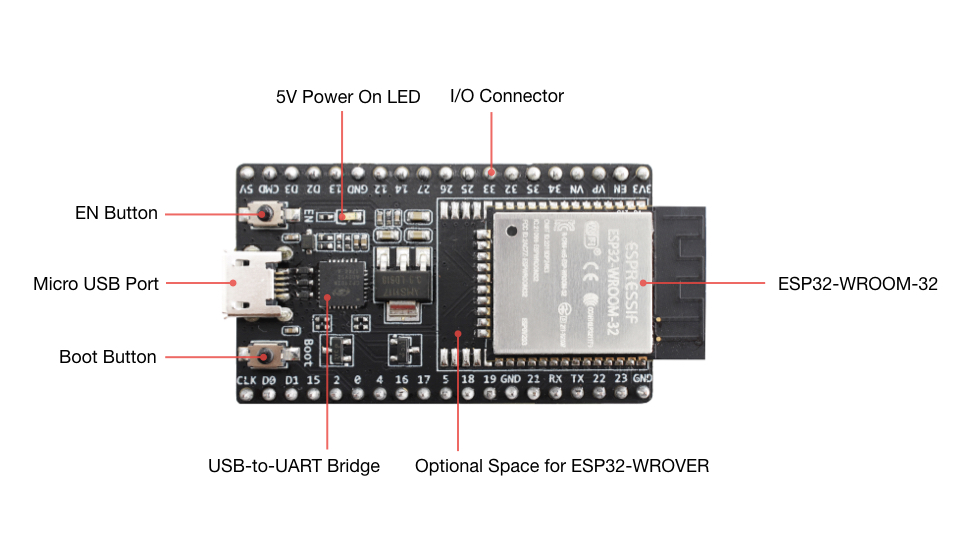
\includegraphics[scale=0.3]{images/esp32-devkitc.jpg}
        \caption{ESP32-DevKitC V4 with ESP32-WROOM-32 module
            \cite{esp32-gettingStarted}}
        \label{esp32_img}
    \end{figure}
    Comme dit plus haut, les noeuds de notre réseau sont des \esp.
    Pour ce projet, nous utilisons un kit de développement (Fig. \ref{esp32_img}) équipé d'un
    \esp\textsc{-wroom32}, développé par Espressif. L'\esp\textsc{-wroom32}
    un System-on-Chip (SoC), c'est à dire un circuit intégré rassemblant plusieurs
    composants comme des entrées/sorties, de la mémoire \textsc{ram}, micorprocesseurs,
    microcontrôleurs, etc.
    %todo prix
    Il a été choisi pour son faible coût (entre 3.50\euro\ et 4\euro) et sa conception adaptée à l'Internet des Objets (IoT). 
    En effet, en plus de supporter le \wifi\ et le Bluetooth 2.4GHz,
    sa consommation en énergie est faible et il possède des mécanismes permettant de l'économiser. %et il possède plusieurs modes de fonctionnement.
    %permettant de la réduire (voir Table \ref{Consumption_PowerModes}).
    La table \ref{spec} fournit ses spécifications.
    \begin{table}[H]
        \centering
        \begin{tabular}{|c|c|}
            \hline
            \rowcolor{lightgray}
            Element & Spécification\\ \hline
            WiFi & 802.11 b/g/n (802.11n jusqu'à 150 Mbps)\\ \hline
            Bluetooth & Bluetooth v4.2 BR/EDR and BLE specification\\ \hline
            CPU & 2 micorprocesseurs Xtensa \up{\tiny{\textregistered}} 32-bit LX6\\ \hline
            Interfaces & \makecell{SD card, UART, SPI, SDIO, I2C, LED PWM, Motor PWM, I2S,IR, \\
                pulse counter, GPIO, capacitive touch sensor, ADC, DAC}\\ \hline
            \makecell{Tension de \\fonctionnement} & $3.0V \sim 3.6V$\\ \hline
        \end{tabular}
        \caption{Spécification de l'\esp\textsc{-wroom32} \cite{esp32-WROOM-32-datasheet}}
        \label{spec}
    \end{table}
    \textbf{Schéma-bloc}
    \begin{figure}[H]
        \centering
        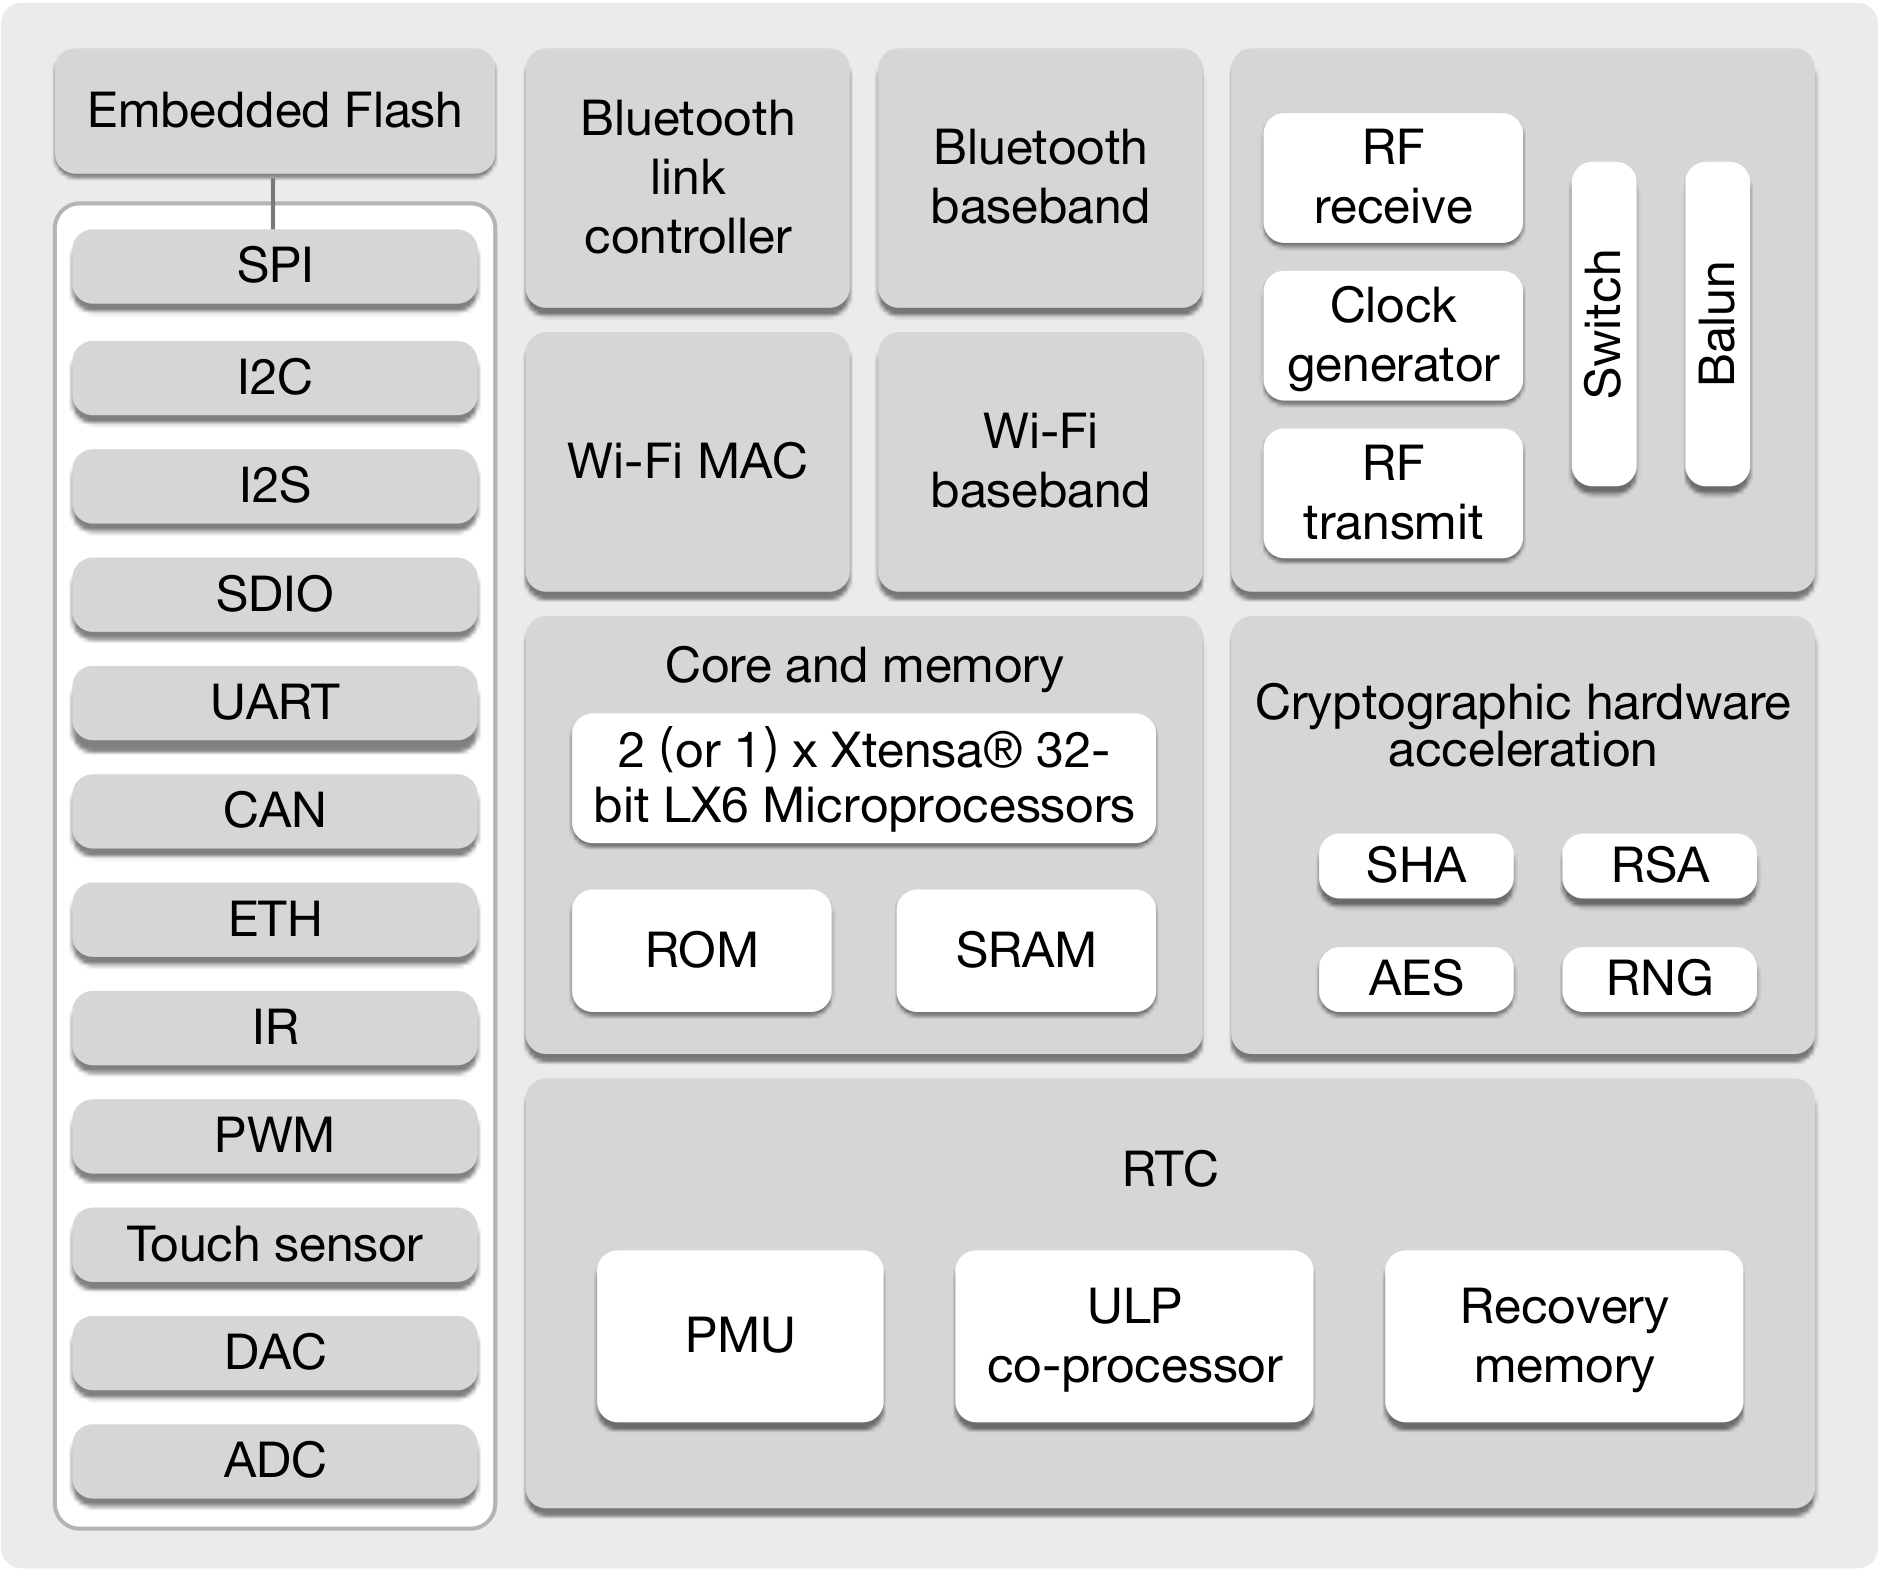
\includegraphics[scale=0.15]{images/esp32-blockDiagram.png}
        \caption{Schéma-bloc \cite{esp32-datasheet}}
        %\label{}
    \end{figure}

    \textbf{Mémoire}\cite{esp32-WROOM-32-datasheet}\\
        La mémoire interne inclut:
        \begin{itemize}
            \item 448 KB de ROM pour le démarrage et les fonctions de base
            \item 520 KB de SRAM pour les données et les instructions
        \end{itemize}
        L'\esp\ prend aussi en charge de la mémoire externe.\\
    
    
        \textbf{Gestion de l'énergie}\\
        Comme dit plus haut, l'\esp\ a une consommation d'énergie faible. De plus, il possède plusieurs
        modes de fonctionnement repris dans la Table \ref{Consumption_PowerModes}, permettant de
        la diminuer.
    
    \begin{table}[H]
        \centering
        \begin{tabular}{|l|c|l|}
            \hline
            \rowcolor{lightgray}
            Power mode & Description & Power consumption\\\hline
            Active & radio and CPU are on  & 95mA $\sim$ 240 mA\\ \hline
            Modem-sleep & radio is off, CPU is on at 80MHz & 20mA $\sim$ 31mA\\ \hline
            Light-sleep & \makecell{CPU is paused, RTC memory and \\peripherals are running.\\
            Any wake-up events like \mac\ events will \\wake
            up the chip.} & 0.8mA\\ \hline
            Deep-sleep & RTC memory and RTC peripherals are powered on & $10\mu A\sim 150\mu A$\\ \hline
            Hibernation & RTC timer only & $5\mu A$\\ \hline
            Power off & - & $0.1 \mu A$\\ \hline
        \end{tabular}
        \caption{Consommation par mode \cite{esp32-datasheet}}
        \label{Consumption_PowerModes}
        
    \end{table}





    %L'\esp\ est un système embarqué développé par Espressif et dédié à l'internet
    %des objets.\\
    %Il est compatible WiFi et Bluetooth 2.4 GHz. Il a une consommation faible
    %en énergie et des mécanismes d'économies d'énergie.\\
    %Il est équipé de 34 pins GPIOs, d'un CPU Xtensa \up{\tiny{\textregistered}}
    %single-/dual-core 32-bit LX6
    %\begin{figure}[H]
    %    \centering
    %    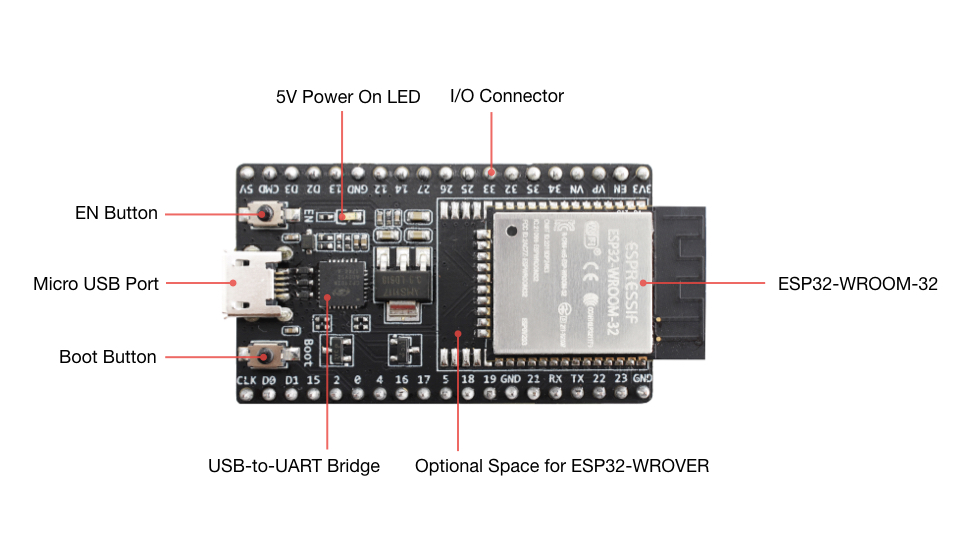
\includegraphics[scale=0.4]{images/esp32-devkitc.jpg}
    %    \caption{ESP32-DevKitC V4 with ESP32-WROOM-32 module
    %        \cite{esp32-gettingStarted_w}}
    %    \label{esp32_img}
    %\end{figure}

%%%%%%%%%%%%%%%%%%%%%%%%%%%%%%%%%%%%%%%%%%%%%%%%%%%%%%%%%%%%%%%%%%%%%%%%%%%%%%%
\section{Environnement de développement}
    Trois environnements s'offrent à nous:
    \begin{enumerate}
        \item \textbf{MicroPython}\cite{micropython}\\
            Selon le site officiel de MicroPython, MicroPython
            est une implémentation simple et efficace de Python 3 incluant un
            petit sous-ensemble de la bibliothèque standard Python. Il est
            optimisé pour fonctionner sur des microcontrôleurs, open source et facile à utiliser.
            La documentation est complète et de nombreux tutoriels sont disponible et facilement compréhensible.
            Cependant, MicroPython n'expose pas les fonctions de bas niveau utiles pour ce projet.
            Par exemple il semble difficile d'envoyer des paquets au niveau de la
            couche lisaison de données ou encore, d'avoir accès aux tables de routages \textsc{ip}.\\
            Voici un exemple illustrant la simplicité du langage. Cet exemple permet de faire clignoter
            une led branchée au \textsc{gpio} 23.
            \begin{minted}[frame=lines,framesep=2mm,baselinestretch=1.2,bgcolor=myGray,fontsize=\footnotesize, linenos]{python}
import machine
import time
led = machine.Pin(23, machine.Pin.OUT) #led configuration
while(TRUE):
    led.value(1) #led on
    time.sleep(1) # delay
    led.value(0) #led off
    time.sleep(2)
            \end{minted}
        
        \item \textbf{IoT Development Framework (IDF)}\cite{idf}\\
            IDF est l'environnement du constucteur de l'\esp\ (Espressif).
            La documentation est complète mais le code source n'est pas entièrement
            disponible. Pour certaines parties du framework, nous n'avons accès qu'aux
            fichiers d'entête.
            Ce framework est natif et nous apportera donc une plus grande fidélité à l'\esp.
            Cet environnement nous donne aussi accès à des fonctionnalités de FreeRTOS
            (free real-time operating system), un système d'exploitation temps
            réel open source pour microcontrôleurs. Ses fonctionnalités pourront nous être 
            utiles pour ce projet. 
            Des protocoles tel que \espmesh\ ou
            \espnow\ sont également disponible. Ils faciliteraient la mise en place d'un réseau \mesh.
            Voici un exemple de code permettant de faire clignoter une led.
            \begin{minted}[frame=lines,framesep=2mm,baselinestretch=1.2,bgcolor=myGray,fontsize=\footnotesize, linenos]{c}
            #include <stdio.h>
            #include "freertos/FreeRTOS.h"
            #include "freertos/task.h"
            #include "driver/gpio.h"
            #include "sdkconfig.h"

            #define BLINK_GPIO CONFIG_BLINK_GPIO
            
            void app_main(void)
            {
                /*Configure the IOMUX register for pad BLINK_GPIO*/
                gpio_pad_select_gpio(BLINK_GPIO);
                /* Set the GPIO as a push/pull output */
                gpio_set_direction(BLINK_GPIO, GPIO_MODE_OUTPUT);
                while(1) {
                    /* Blink off (output low) */
                    printf("Turning off the LED\n");
                    gpio_set_level(BLINK_GPIO, 0);
                    vTaskDelay(1000 / portTICK_PERIOD_MS);
                    /* Blink on (output high) */
                printf("Turning on the LED\n");
                    gpio_set_level(BLINK_GPIO, 1);
                    vTaskDelay(1000 / portTICK_PERIOD_MS);
                }
            }
            \end{minted}
        \item \textbf{Arduino}\cite{aruino-esp32}\\
            L'environnement Arduino se base sur IDF. Il est donc possible que certaines
            fonctionnalités d'IDF ne soient pas disponible. 
            La documentation est moins complète qu'IDF mais tout le code source est disponible.
            Comme MicroPython, il semble difficile d'envoyer des paquets au niveau de la
            couche lisaison de données ou d'avoir accès aux tables de routages \textsc{ip}.\\
            \begin{minted}[frame=lines,framesep=2mm,baselinestretch=1.2,bgcolor=myGray,fontsize=\footnotesize, linenos]{c}
#define LED  2
 
 void setup() {
   pinMode(LED,OUTPUT);
 }
  
 void loop() {
   delay(1000);
   digitalWrite(LED,HIGH);
   delay(100);
   digitalWrite(LED,LOW);
 }

            \end{minted}
    \end{enumerate}
    \vspace{1cm}
    Notons que les solutions évoquées ci-dessus sont gratuites. Il existe des solutions
    commerciales payantes que nous n'avons pas évoqué car il est tout a fait possible de
    travailler avec des solutions gratuites.\\
    
    Nous choisirons IDF pour sa documentation complète, sa nativité et pour son ensemble
    de fonctionnalités plus exhaustif que les autres environnements. Néanmoins, 
    avec les extraits de code, nous remarquons qu'il sera plus difficile à prendre en mains.

%%%%%%%%%%%%%%%%%%%%%%%%%%%%%%%%%%%%%%%%%%%%%%%%%%%%%%%%%%%%%%%%%%%%%%%%%%%%%%%
\section{Protocoles de routage}
    Dans cette section, nous discutons de différents protocoles de routage envisageables.
    Nous allons d'abord établir un classement des protocoles de routage \mesh.
    Ensuite nous allons décrire brièvement les protocoles les plus cités dans la littérature pour les classer
    en fonction de leur appartenance à une catégorie établie dans notre classement. 
    Enfin, nous allons choisir un protocole à implémenter pour ce projet.\\

    \underline{\textbf{Classification}}\\

    Les protocoles de routages \mesh\ peuvent être divisés en deux grandes catégories:
    \begin{enumerate}
        \item \textbf{Proactifs}: Les noeuds maintiennent une/des table(s) de routage
            qui stockent les routes vers tous les noeuds du réseau. 
            Ils envoient régulièrement des paquets de contrôle à travers le réseau pour échanger et 
            mettre à jour l'information de leurs voisins.
        \item \textbf{Réactifs}: Ces protocoles établissent une route uniquement quand des paquets
            doivent être transférés.
    \end{enumerate}
    Nous écartons les protocoles proactifs pour ce projet car ils gardent
    beaucoup d'information en mémoire. Ils ne passent donc pas à l'échelle.
    Les protocoles réactifs sont plus économes en ressources, mais nécessitent parfois un délai
    plus long pour établir une route, car elles sont établies à la demande.\\

    \underline{\textbf{Description}}\\

    Il existe une multitude de protocols de routage \mesh.
    Ci-dessous, en voici quelques-uns souvent cités dans la littérature:\\
    \begin{itemize}
        \item \textbf{AODV}\cite{rfc_aodv} Ad-hoc On-demand Distance Vector\\
            Protocole réactif à vecteur de distance que nous décrirons en détail par la suite.\\
        \item \textbf{DSR}\cite{rfc_dsr} Dynamic Source Routing\\
            Similaire à AODV mais ici, les paquets servant à la découverte d'un chemin
            (\textit{RREQ}) contiennent tous les sauts de ce chemin.\\
        \item \textbf{OLSR}\cite{rfc_olsr} Optimized Link State Routing\\
            Protocole proactif à état de liens. Dans ce protocole, certains noeuds servent de relais pour effectuer
            le broadcasting des paquets servant à la découverte de chemins. L'ensemble de ces noeuds forme un arbre couvrant du réseau.\\
        \item \textbf{B.A.T.M.A.N}\cite{batman} Better Approach to Mobile Adhoc Networking\\
            Protocole proactif à état de liens. Le protocole ne calcule
            pas le chemin pour atteindre un noeud mais le meilleur saut dans la bonne direction.
            Pour cela, pour chaque destination il va sélectionner son voisin qui lui a transmis
            le plus de messages de cette destination.\\
        \item \textbf{DSDV}\cite{dsdv} Destination Sequence Distance Vector\\
            Protocole à vecteur de distance basé sur l'algorithme de Bellman-Ford.
    \end{itemize}

    Nous pouvons donc classer ces protocoles de la manière suivante: 
    \begin{diagram}[H]
        \Tree[.{wireless network protocols} 
            [.Reactive [.\textsc{aodv} ]
                [.\textsc{dsr} ]]
            [.Proactive [.{Link-state} 
                [.\textsc{olsr} ] 
                [.\textsc{b.a.t.m.a.n} ]] 
                [.{Distance-vector} [.\textsc{dsdv} ]]]]
        \caption{Classifications des protocols de routage }
    \end{diagram}

    \underline{\textbf{Choix d'un protocole}}\\

    Comme dit plus haut, nous écartons les protocoles proactifs. Il nous reste donc le choix entre \aodv\ et \textsc{dsr}.
    Nous allons retenir \aodv\ pour la taille fixe de ses paquets. En effet, \textsc{dsr} utilise plus de données quand
    les routes contiennent un grand nombre de sauts.

    
    
%    Dans cette section nous discutons de différents protocoles de routage envisageables.\\
%    Tout d'abord, nous établirons un classement des différents types de protocoles de routage\mesh. \\
%    Ensuite, nous etudierons et comparerons différents protocoles de routage mesh: \espmesh\
%    \cite{esp-mesh_w}, OLSR\cite{olsr_w}, AODV\cite{aodv_w} et DSR\cite{dsr_w}\\
%    Enfin nous allons choisir un protocole à implémenter sur \esp.\\
%    
%    \subsection{Classification}
%    Les protocoles de routages \mesh\ peuvent être divisés en deux grandes catégories:
%    \begin{enumerate}
%        \item \textbf{Proactifs}: Les noeuds maintiennent une/des table(s) de routage
%            qui stockent les routes vers tous les noeuds du réseau. 
%            Ils envoient régulièrement des paquets de contrôle à travers le réseau pour échanger et 
%            mettre à jour l'information de leurs voisins.
%        \item \textbf{Réactifs}: Ces protocoles établissent une route uniquement quand des paquets
%            doivent être transférés.
%    \end{enumerate}
%    Nous écarterons les protocoles proactifs pour ce projet car ils gardent
%    beaucoup d'information en mémoire. Ils ne passent donc pas à l'échelle.\\
%    Les protocoles réactifs sont plus économes en ressources mais nécessitent parfois un délai
%    plus long pour établir une route
%    car elles sont établies à la demande.\\
%    
%    Il existe une multitude de protocols de routage \mesh. 
%    Ci-dessous, en voici quelques-uns souvent cités dans la littérature:\\
%    \begin{itemize}
%        \item \textbf{AODV}\cite{aodv_w} Ad-hoc On-demand Distance Vector\\
%            Protocole réactif à vecteur de distance que nous décrirons en détail par la suite.\\
%        \item \textbf{DSR}\cite{dsr_w} Dynamic Source Routing\\
%            Similaire à AODV mais ici, les paquets servant à la découverte d'un chemin
%            (\textit{RREQ}) contiennent tous les sauts de ce chemin.\\
%        \item \textbf{OLSR}\cite{olsr_w} Optimized Link State Routing\\
%            Protocole proactif à état de liens. Dans ce protocole, certains noeuds servent de relais pour effectuer
%            le broadcasting des paquets servant à la découverte de chemins. L'ensemble de ces noeuds forme un arbre couvrant du réseau.\\
%        \item \textbf{B.A.T.M.A.N}\cite{batman_w} Better Approach to Mobile Adhoc Networking\\
%            Protocole proactif à état de liens. Le protocole ne calcule
%            pas le chemin pour atteindre un noeud mais le meilleur saut dans la bonne direction.
%            Pour cela, pour chaque destination il va sélectionner son voisin qui lui a transmis
%            le plus de messages de cette destination.\\
%        \item \textbf{DSDV}\cite{dsdv_w} Destination Sequence Distance Vector\\
%            Protocole à vecteur de distance basé sur l'algorithme de Bellman-Ford.
%    \end{itemize}
%    On peut donc classer ces protocoles de la manière suivante: 
%    \begin{diagram}[H]
%        \Tree[.{wireless network protocols} 
%            [.Reactive [.\textsc{aodv} ]
%                [.\textsc{dsr} ]]
%            [.Proactive [.{Link-state} 
%                [.\textsc{olsr} ] 
%                [.\textsc{b.a.t.m.a.n} ]] 
%                [.{Distance-vector} [.\textsc{dsdv} ]]]]
%        \caption{Classifications des protocols de routage }
%    \end{diagram}
%
%
%%%%%%%%%%%%%%%%%%%%%%%%%%%%%%%%%%%%%%%%%%%%%%%%%%%%%%%%%%%%%%%%%%%%%%%%%%%%%%%
%\chapter{ESP MESH}
        \espmesh\ est le protocole du constructeur Espressif permettant d'établir un réseau mesh avec des \esp.
        Cette section explique le fonctionnement de ce protocole. \espmesh\ a pour objectif la création d'un arbre recouvrant.
        Il existe plusieurs types de noeuds:
        \begin{enumerate}
            \item \textbf{Racine}: seule interface entre le réseau \espmesh\ et un réseau \textsc{ip} externe.
            \item \textbf{Noeuds intermédiaires}: noeuds qui ont un parent et au moins un enfant.
            Ils transmettent leurs paquets et ceux de leurs enfants.
            \item \textbf{Feuilles}: noeuds qui n'ont pas d'enfants et ne transmettent que leurs paquets.
            \item \textbf{Noeuds idle}: noeuds qui n'ont pas encore rejoint un réseau \espmesh.
        \end{enumerate}

        \begin{figure}[H]
            \centering
            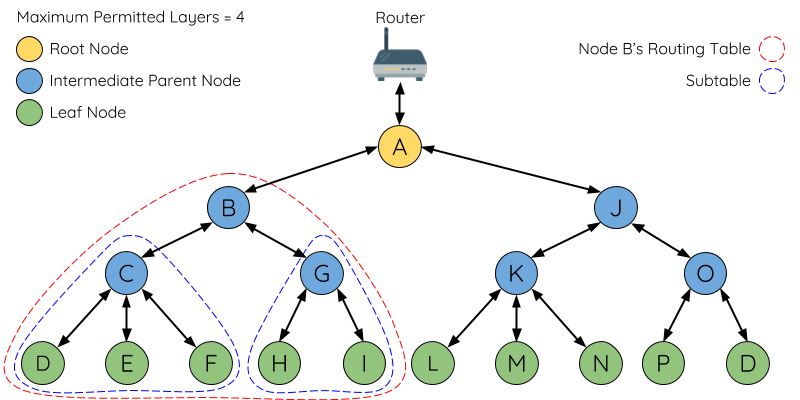
\includegraphics[scale=0.3]{images/mesh-node-types.png}
            \caption{Topologie d'un réseau \espmesh \cite{esp-mesh_w}}
        \end{figure}

        \textbf{Routage}\newline
        \begin{itemize}
            \item Table de routage\\
                Chaque noeud possède sa table de routage. Soit $p$ un noeud, sa table de routage contient les adresses \mac\ 
                des noeuds du sous-arbre ayant $p$ comme racine, et également celle de $p$.\\
                Elle est partitionnée en sous-tables qui correspondent aux sous-arbres des enfants de $p$.
                Par exemple, nous pouvons apercevoir sur la figure précédente, la table de routage du noeud B (en rouge).
                Elle est partitionnée en 2 sous-table (en bleu) contenant respectivement les noeuds C, D, E, F et G, H, I.
            \item Acheminement de paquets\\
                Quand un paquet est reçu,
                \begin{itemize}
                    \item Si l'adresse \mac\ du paquet est dans la table de routage et si elle est différente de l'adresse du noeud l'ayant reçu, le paquet est envoyé
                    à l'enfant correspondant à la sous-table contenant l'adresse.
                    \item Si l'adresse n'est pas dans la table de routage, le paquet est envoyé au parent.
                \end{itemize}
                %\espmesh\ utilise un mécanisme de vérification de chemin pour détecter les boucles. Si une boucle arrive, un parent va prévenir son enfant et initier une déconnexion.

        \end{itemize}
        \vspace{0.5cm}

        \textbf{Construction d'un réseau}
        \newline
        \begin{enumerate}
            \item \'Election de la racine
                \begin{itemize}
                    \item \textbf{Sélection automatique}\\
                        Chaque noeud idle va transmettre son adresse \mac\ et
                        la valeur de son \rssi\ (Received Signal Strength Indication) avec le routeur via des beacons.
                        Dans le but de choisir comme racine, le noeud le plus proche de l'AP.
                        Simultanément, chaque noeud scanne les beacons des autres noeuds. Si un noeud
                        en détecte un autre avec un \rssi\ strictement plus fort, il va transmettre le contenu de
                        ce beacon (càd voter pour ce noeud).
                        Ce processus sera répété pendant un nombre minimum d'itérations (10 par défaut).
                        Une itération pour un noeud, consiste à avoir reçu les beacons de tous les autres noeuds
                        et avoir voté pour le noeud ayant le meilleur \rssi\ avec le routeur.
                        Après toutes les itérations, chaque noeud va calculer le ratio suivant: 
                        \[\frac{nombre\ de\ votes\ pour\ ce\ noeud}{nombre\ de\ noeuds\ participants\ \textrm{\textit{à l'élection}}}\]
                        Cest deux informations sont connues par la réception des beacons.
                        Si ce ratio est au-dessus d'un certain seuil (par défaut 90\%), ce noeud deviendra la racine.\footnote{
                            Si plusieurs racines sont élues, deux réseaux \espmesh\ seront créés.
                            Dans ce cas, \espmesh\ possède un mécanisme interne (dont le fonctionnement n'est pas décrit par Espressif) qui va fusionner les deux réseaux
                            ssi les racines sont connectées au même routeur.
                        }



                    \item \textbf{Sélection par l'utilisateur}\\
                        Le choix de la racine peut être réalisé par l'utilisateur via l'\textsc{API} \espmesh.
                        Dans ce cas, la racine se connecte au routeur et elle, ainsi que les autres noeuds, oublient le processus
                        d'élection.
                \end{itemize}
            \item Formation de la deuxième couche\\
                %Une fois le processus d'élection d'une racine terminé, chaque noeud va émettre des beacons
                %pour permettre aux autres noeuds de détecter sa présence et de connaître son statut.
                %Ces beacons contiennent les informations suivantes:
                %\begin{itemize}
                %    \item[$\bullet$] Type du noeud (racine, intermédiaire, feuille, idle)
                %    \item[$\bullet$] Couche sur laquelle se trouve le noeud
                %    \item[$\bullet$] Nombre de couches maximum autorisées dans le réseau
                %    \item[$\bullet$] Nombre de noeuds enfants
                %    \item[$\bullet$] Nombre maximum d'enfants   
                %\end{itemize}
                %Les noeuds idle à portée de la racine vont s'y connecter et devenir des noeuds intermédiaires.
                Une fois le processus d'élection d'une racine terminé,
                les noeuds idle à portée de la racine vont s'y connecter et devenir des noeuds intermédiaires
            
            \item Formation des autres couches\\
                %Les noeuds idle à portée de noeuds intermédiaires vont s'y connecter. 
                Chaque noeud du réseau \espmesh\ émet périodiquement des beacons contenant les
                informations suivantes:
                \begin{itemize}
                    \item[$\bullet$] Type du noeud (racine, intermédiaire, feuille, idle)
                    \item[$\bullet$] Couche sur laquelle se trouve le noeud
                    \item[$\bullet$] Nombre de couches maximum autorisées dans le réseau
                    \item[$\bullet$] Nombre de noeuds enfants
                    \item[$\bullet$] Nombre maximum d'enfants   
                \end{itemize}
                %Sur base de ces beacons, les noeuds idle vont connaître leurs potentiels parents. Si plusieurs parents
                %sont possibles, un noeud choisira son parent selon deux critères connus par les beacons des noeuds intermédiaires.
                Sur base du contenu de ces beacons, les noeuds idle conaissent leurs potientiels parents.
                Si plusieurs parents sont possibles, un noeud choisira son parent selon deux critères:
                \begin{enumerate}
                    \addtolength{\itemindent}{1cm}
                    \item[1.] La couche sur laquelle se situe le candidat parent:
                        le candidat se trouvant sur la couche la moins profonde sera choisi. 
                    \item[2.] Le nombre d'enfants du candidat parent: si plusieurs candidats se trouvent
                        sur la couche la moins profonde, celui avec le moins d'enfants sera choisi. 
                \end{enumerate}
                
                Un noeud peut également se connecter à un parent prédéfini.
                Une fois connectés, les noeuds deviennent des noeuds intermédiaires si le nombre maximal de couches n'est pas atteint.
                Sinon, les noeuds de la dernière couche deviennent automatiquement
                des feuilles, empêchant d'autres noeuds dans l'état idle de s'y connecter.

        \end{enumerate}
        Pour éviter les boucles, un noeud ne va pas se connecter à un noeud dont l'adresse \mac\ se trouve dans sa table de routage.
        \vspace{0.5cm}\\
        \textbf{Mise sous tension asynchrone}\newline
            La structure du réseau peut être affectée par l'ordre dans lequel les noeuds sont mis sous tension.
            Les noeuds ayant une mise en tension retardée suivront les deux règles suivantes:
            \begin{enumerate}
                \item Si le noeud détecte, par les beacons, qu'une racine existe déjà, il ne vas pas essayer
                    d'élire une nouvelle racine
                    même si son \rssi\ avec le routeur est meilleur. Il va rejoindre le réseau comme un noeud idle. \\
                    Si le noeud est la racine désignée, tous les autres noeuds vont rester idle
                    jusqu'à ce que le noeud soit mis sous tension.
                \item Si le noeud devient un noeud intermédiraire, il peut devenir le meilleur parent d'un autre noeud 
                (cet autre noeud changera donc de parent).
                \item Si un noeud idle a un parent prédéfini et que ce noeud n'est pas sous tension, il ne va pas essayer
                de se connecter à un autre parent.
            \end{enumerate}
        \vspace{0.5cm}
        \textbf{Défaillance d'un noeud}\newline
            \begin{itemize}
                \item Défaillance de la racine\\
                    Si la racine tombe, les noeuds de la deuxième couche vont d'abord tenter de s'y reconnecter.
                    Après plusieurs échecs, les noeuds de la deuxième couche vont entamer entre eux le processus d'élection d'une nouvelle racine.
                    Si la racine ainsi que plusieurs couches tombent, le processus d'élection sera initialisé sur la couche la plus haute.


                \item Défaillance d'un noeud intermédiaire\\
                    Si un noeud intermédiaire tombe, ses enfants vont d'abord tenter de s'y reconnecter.
                    Après plusieurs échecs, ils se connecteront au meilleur parent disponible.
                    S'il n'y a aucun parent possible, ils se mettront dans l'état idle.
                    \begin{figure}[H]
                        \centering
                        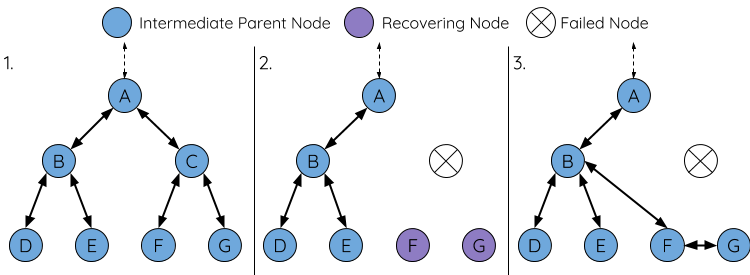
\includegraphics[scale=0.5]{images/mesh-parent-node-failure.png}
                        \caption{Défaillance d'un noeud intermédiaire\cite{esp-mesh_w}}
                    \end{figure}
            \end{itemize}
            \vspace{0.5cm}
            \textbf{Changement de racine}\newline
                Un changement de racine n'est possible que dans deux situations:
                \begin{enumerate}
                    \item La racine tombe. (voir point précédent)
                    \item La racine le demande via un appel à \textbf{esp\_mesh\_waive\_root()}.
                        Dans ce cas, un processus d'élection de racine sera initialisé. La nouvelle racine élue
                        enverra alors une \textit{switch request} à la racine actuelle qui répondra par un acquittement.
                        Ensuite la nouvelle racine se déconnectera de son parent et se connectera au routeur.
                        L'ancienne racine se déconnectera du routeur et deviendra un noeud idle pour enfin se connecter à un nouveau parent.
                \end{enumerate}
        \textbf{Paquets ESP-MESH}\\
            Les paquets \espmesh\ sont contenus dans une trame \wifi. Une transmission multi-sauts utilisera un paquet \espmesh\ transporté 
            entre chaque noeud par une trame \wifi\ différente.
            La figure \ref{fig_meshPacket} montre la structure d'un paquet \espmesh:\\

            \begin{figure}[h]
                \centering
                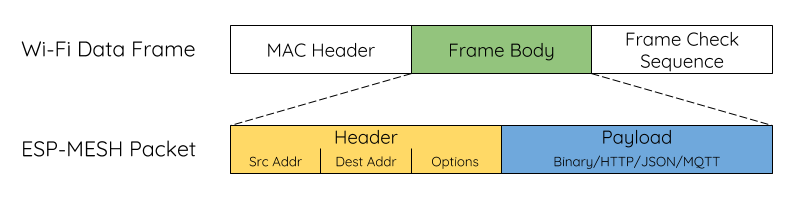
\includegraphics[scale=0.5]{images/mesh-packet.png}
                \caption{Paquet \espmesh\ \cite{esp-mesh_w}}
                \label{fig_meshPacket}
            \end{figure}
            Le header d'un paquet \espmesh\ contient les adresses source et destination ainsi que diverses options.
            Le payload d'un paquet \espmesh\ contient les données de l'application.

            Dans le cas où l'adresse de destination est une adrese \textsc{ip}, le paquet sera envoyé à la racine du réseau
            \espmesh\ qui transmet le payload du paquet (par exemple en initiant une connexion tcp avec un socket).
        \vspace{0.5cm}\\
        \textbf{Contrôle de flux}\\
            Pour éviter que les parents soient submergés de flux venant de leurs enfants, chaque parent va
            assigner une fenêtre de réception à chaque enfant. Chaque noeud enfant doit demander une fenêtre
            de réception avant chaque transmission. La taille de la fenêtre peut être ajustée dynamiquement.
            Une transmission d'un enfant vers un parent se déroule en plusieurs étapes:
            \begin{enumerate}
                \item Le noeud enfant envoit à son parent une requête de fenêtre. Cette requête contient le numéro de séquence du paquet en attente d'envoi.
                \item Le parent reçoit la requête et compare le numéro de séquence avec celui du précédent paquet envoyé par l'enfant.
                    La comparaison est utilisée pour calculer la taille de la fenêtre qui est transmise à l'enfant.\footnote{Ce calcul n'est pas précisé par Espressif}
                \item L'enfant transmet le paquet conformément à la taille de fenêtre spécifiée par le parent. Une fois la fenêtre de réception utilisée, l'enfant doit renvoyer une demande de fenêtre.
            \end{enumerate}
        \vspace{0.5cm}
        \textbf{Performances}\\
            Espressif fournit les performances d'\espmesh\ pour un réseau de maximum 100 noeuds, 6 couches et
            un nombre d'enfants par noeud de 6 (voir table \ref{performances_espMesh}).
            \begin{table}[H]
                \begin{tabular}{|l|l|}
                    \hline
                    Temps de construction du réseau & $<$ 60 secondes\\ \hline
                    Latence par saut & 10 à 30 millisecondes\\ \hline
                    Temps de réparation du réseau & \makecell{Si la racine tombe: $<$ 10 secondes \\ Si un noeud enfant tombe: $<$ 5 secondes}\\ \hline
                \end{tabular}
                \caption{Performances d'\espmesh\ \cite{esp-mesh_w}}
                \label{performances_espMesh}
            \end{table}
            \hspace{-0.75cm}
            \textbf{Discussion}\\
            A première vue, une topologie en arbre n'est pas robuste car si la racine tombe,
            tout le reste du réseau est déconnecté. Cependant le processus d'élection
            d'une nouvelle racine semble efficace selon les résulats fournis par Espressif.
            Un point négatif du protocole est que pour un noeud donné, sa table de routage contient tous les
            noeuds de son sous-arbre.
            On imagine donc difficilement utiliser ce protocole pour un nombre élevé de noeuds.    
%    \vspace{1cm}
%%%%%%%%%%%%%%%%%%%%%%%%%%%%%%%%%%%%%%%%%%%%%%%%%%%%%%%%%%%%%%%%%%%%%%%%%%%%%%% 
%\newpage 
%\chapter{AODV}
    Ad-hoc On-demand Distance Vector (\aodv) est un protocole réactif à vecteur de distance.
    Les 3 types de messages définis dans \aodv\ sont les Route requests (\textit{\rreq s}),
    les Route Remplies (\textit{\rrep s}) et les Route Errors (\textit{\rerr s}).
    Comme illustré sur la figure suivante, le premier sera envoyé en flooding par un noeud
    désirant obtenir une nouvelle route pour
    une desination donnée. Le second sert de réponse au premier. Il est envoyé à l'émetteur du
    \rreq. Et le dernier sert notamment lorsqu'un lien d'une route active est brisé. 
    Nous détaillons plus bas ces mécanismes.
    \vspace{1cm}
    \begin{figure}[H]
        \centering
        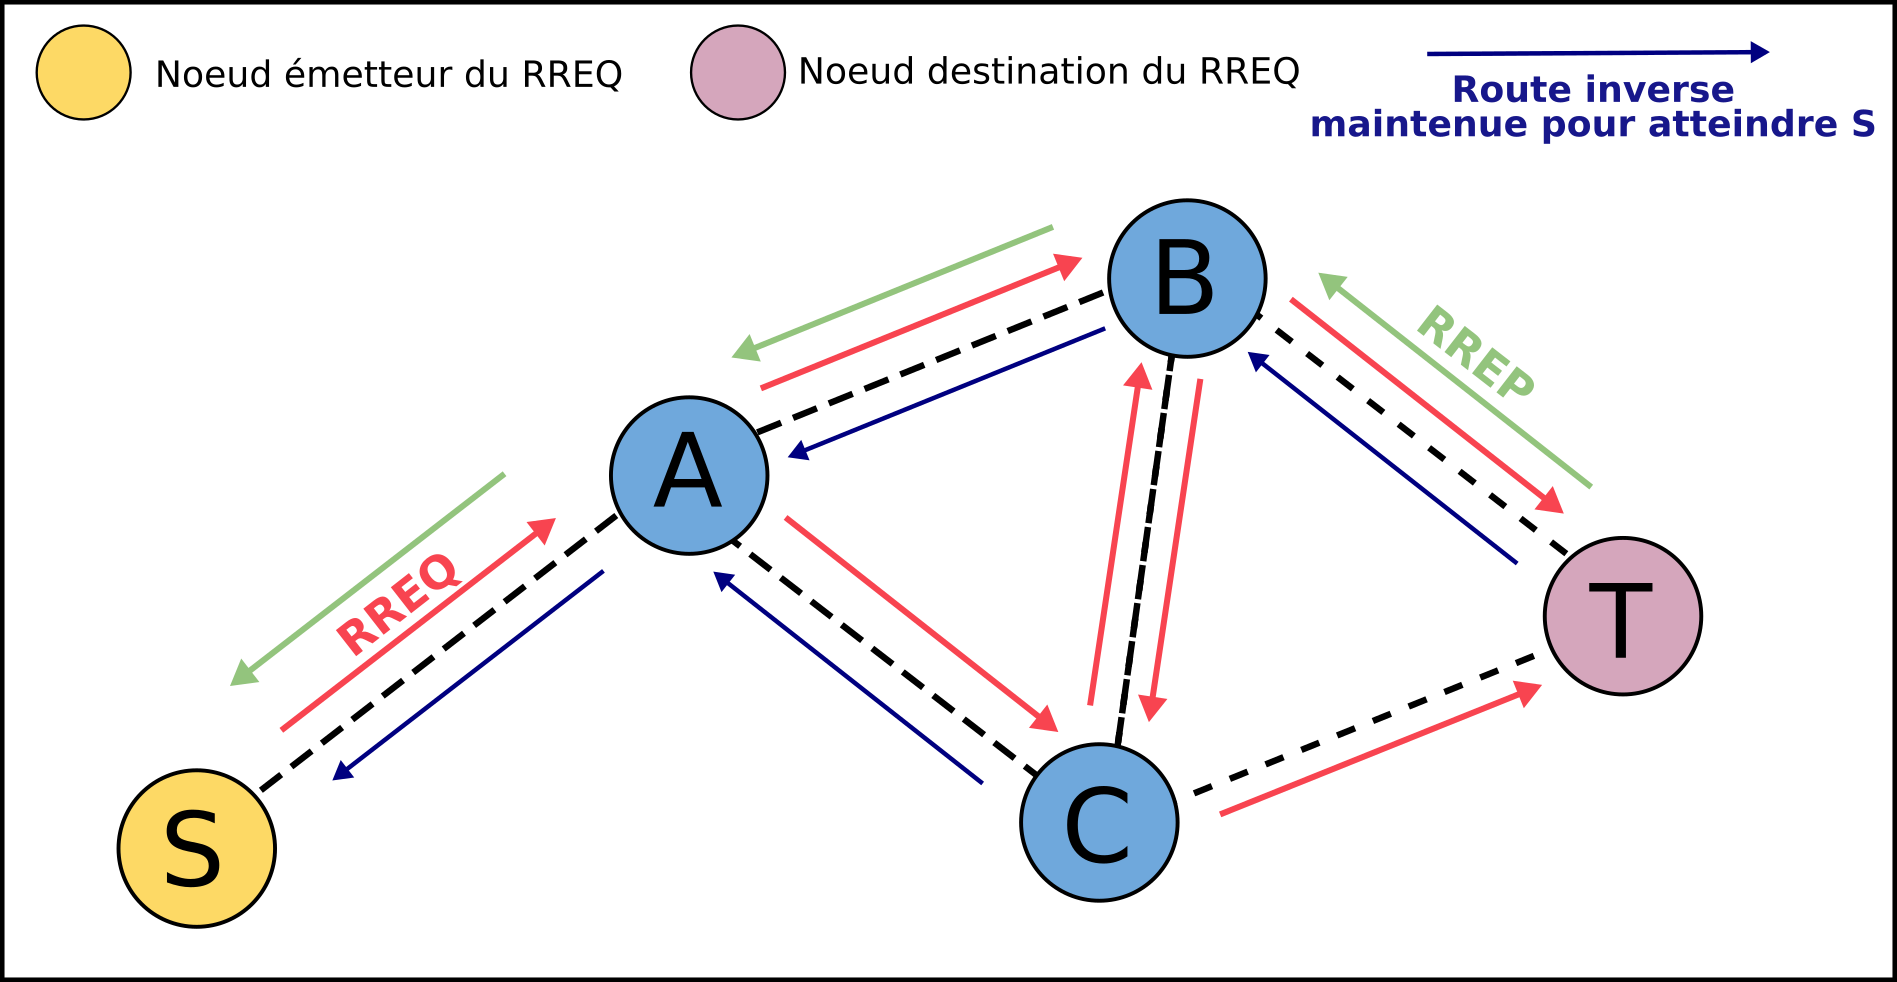
\includegraphics[scale=0.35]{images/aodv.png}
        \caption{Illusration du fonctionnement d'AODV}
        \label{aodv}
    \end{figure}
    
    
    \vspace{0.5cm}
    %\textbf{Format des paquets}\\
    \section{Format des paquets}
        \textbf{RREQ}\\
            \begin{figure}[H]
                \centering
                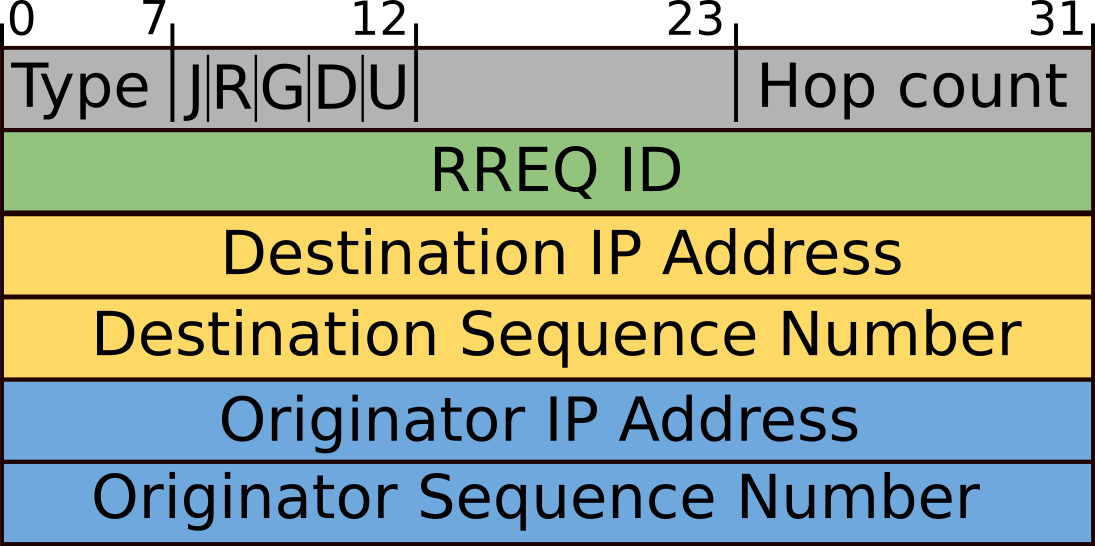
\includegraphics[scale=0.5]{images/rreq.png}
                \caption{Format d'un paquet \rreq\ \cite{rfc_aodv}}
                \label{rreqPaquet}
            \end{figure}
            Le format d'un \rreq\ est illustré sur la figure précédente. Il contient les champs
            repris dans la table suivante:\\
            \begin{table}[H]
                \begin{tabular}{ll}
                    type & \makecell[l]{$=1$}\\\hline
                    J R G & \makecell[l]{flags}\\\hline
                    D  & \makecell[l]{flag indiquant que seul la destination peut\\ répondre au \rreq}\\\hline
                    U & \makecell[l]{flag indiquant que le numéro de séquence de la\\ destination est inconnu}\\\hline
                    Hop count & \makecell[l]{nombre de sauts depuis le noeud source}\\\hline
                    \rreq\ \textsc{id} & \makecell[l]{numéro de séquence identifiant le \rreq}\\\hline
                    Destination IP Address & \makecell[l]{adresse \textsc{ip} du noeud pour lequel la route\\ est demandée}\\\hline
                    Destination Sequence Number & \makecell[l]{le dernier numéro de séquence connu pour une \\route vers la destination}\\\hline
                    Originator IP Address & \makecell[l]{adresse ip de l'émetteur du \rreq}\\\hline
                    Originator Sequence Number & \makecell[l]{numéro de séquence à utiliser pour une route\\ pointant vers l'émetteur du \rreq}\\
                \end{tabular}
                \caption{Champs d'un \rreq\ \cite{rfc_aodv}}
                \label{rreq_fields}
            \end{table}
            
        \textbf{RREP}\\
            \begin{figure}[H]
                \centering
                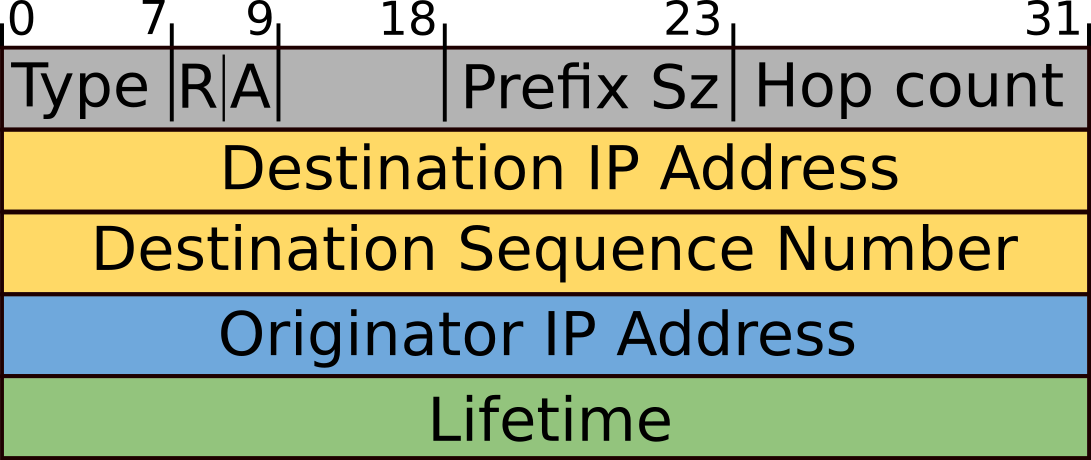
\includegraphics[scale=0.5]{images/rrep.png}
                \caption{Format d'un \rrep\ \cite{rfc_aodv}}
                \label{rreqPaquet}
            \end{figure}
            Le format d'un \rrep\ est illustré sur la figure précédente. Il contient les champs
            repris dans la table suivante:\\
            \begin{table}[H]
                \begin{tabular}{ll}
                    type & \makecell[l]{$=2$}\\ \hline
                    R & \makecell[l]{flag utilisé pour le multicast}\\ \hline
                    Prefix size & \makecell[l]{utilisé pour les aggrégations de routes}\\ \hline
                    Hop Count & \makecell[l]{nombre de sauts de l'\textit{originator} à la destination}\\ \hline
                    Destination IP address & \makecell[l]{adresse IP de du noeud pour qui l'adresse \\est demandée}\\ \hline
                    Destination Sequence Number & \makecell[l]{numéro de séquence de destination \\associé à la route}\\ \hline
                    Originator IP address & \makecell[l]{adresse IP du noeud émetteur du \rreq}\\ \hline
                    Lifetime & \makecell[l]{temps (en ms) pendant lequel le noeud qui reçoit \\le \rrep\ va considérer la route valide}\\
                \end{tabular}
                \caption{Champs d'un \rrep\ \cite{rfc_aodv}}
                \label{rrep_fields}
            \end{table}

    %\textbf{Découverte d'un chemin}\\
    \section{Découverte d'un chemin}
        La découverte d'un chemin est intiée par un noeud voulant envoyer des paquets à une destination pour laquelle il n'a aucune route valide.
        Chaque noeud possède deux compteurs: \textit{sequence\_number} et \textit{rreq\_id}.
        
        
        \vspace{0.5cm}
        \textbf{Génération du RREQ}\\
            Le noeud source incrémente ses compteurs \textit{sequence\_number} et \textit{rreq\_id} de 1.
            Il envoie ensuite un \rreq\ en broadcast à ses voisins.
        
        
        \vspace{0.5cm}
        \textbf{Propagation du RREQ}\\
            \begin{itemize}
                \item[$\bullet$] Noeud intermédiaire\\
                    A la réception d'un \rreq, un noeud intermédiaire va pouvoir rajouter ou mettre à jour
                    les routes vers son prédécesseur et vers le noeud source du \rreq.\\
                    Ensuite deux situations sont possibles:
                    \begin{enumerate}
                        \item Le noeud courant possède une route active vers la destination et le numéro de séquence de la route est plus grand 
                            ou égal au numéro de séquence de la destination dans le \rreq.
                            Dans ce cas, il peut envoyer par unicast un \rrep\ à la source du \rreq.
                        \item Sinon\\
                            Le noeud va incrémenter le nombre de sauts du \rreq\ et le propager à ses voisins.
                    \end{enumerate}

                \item[$\bullet$] Noeud destination\\
                    A la réception d'un \rreq\  lui étant destiné, un noeud va, comme un noeud intermédiaire, 
                    rajouter ou mettre à jour les routes vers son prédécesseur et vers le noeud source du \rreq.
                    Si le \textit{Destination Sequence Number} du \rreq\ est égal à son \textit{sequence\_number},
                    il va incrémenter ce dernier et envoyer un \rrep\ en unicast vers la source du \rreq.     
            \end{itemize}

        \vspace{0.5cm}
        \textbf{Propagation du RREP}\\
            A la réception d'un \rrep\ , un noeud va pouvoir rajouter ou mettre à jour
            les routes vers le noeud source du \rrep\  et vers son successeur.\\
            Il va ensuite incrémenter le nombre de sauts du \rrep\  et le propager en unicast vers la destination de ce \rrep\ .
            Cette propagation en unicast vers la source du \rreq\ est possible par l'apprentissage de la route inverse
            (destination du \rreq\ vers l'émetteur du \rreq) réalisée lors du flooding du \rreq.

    %\underline{\textbf{Table de routage}}\\
    \section{Table de routage}
        Chaque entrée d'une table de routage contient les informations suivantes:
        
        \begin{table}[H]
            \centering
            \begin{tabular}{|l|l|}
                \hline
                \textit{dest}       & Adresse IP de destination\\
                \textit{dest\_SN}   & Numéro de séquence de destination\\
                \textit{flag}       & Indicateur de numéro de séquence de destination valide\\
                \textit{out}        & Interface réseau\\
                \textit{hops}       & \makecell[l]{Comptage de sauts (nombre de sauts nécessaires\\ pour atteindre la destination)}\\
                \textit{next-hop}   & Prochain saut\\
                \textit{precursors} & Liste des précurseurs\\
                \textit{lifetime}   & temps d'expiration ou de suppression de l'itinéraire\\
                \hline
            \end{tabular}
            \caption{entrée d'une table de routage \aodv \cite{rfc_aodv}}
            \label{routingTable_aodv}
        \end{table}

        \textbf{Mise à jour de la table de routage}\\
            Soit N une nouvelle route et O la route existante.\\
            O est mise à jour si:\\
            \begin{center}
                \begin{tabular}{|l|}
                    \hline
                    $O.SN \leq N.SN$ \\
                    \textbf{ou} ($O.SN = N.SN$ \textbf{et} $O.hop\_count > N.hop\_count$)\\
                    \hline
                \end{tabular}
            \end{center}
        
        \textbf{Gestion du \textit{lifetime}}\\
            Le temps de vie d'une route dans la table de routage est initialisé à \textit{active\_route\_timeout} (3 millisecondes).\\
            Quand ce timer expire, la route passe de active à inactive. Une route inactive ne pourra plus être utilisée pour transférer des données
            mais pourra fournir des informations pour de futurs \rreq\  et la réparation de routes.\\
            Quand une route est utilisée, son temps de vie  est actualisé à: $current time + active\_route\_timeout$

    %\vspace{0.5cm}
    %\textbf{Evitement de boucles}\\
    \section{Evitement de boucles}
        A priori les numéros de séquences suffisent pour éviter les boucles. Cependant, d'après \cite{loop_aodv}, il y a des
        ambiguités dans le RFC \cite{rfc_aodv}. Dû à ces ambiguités, l'implémentation pourrait introduire des boucles.
        %Certaines parties du RFC concerant la gestion des numéros de séquences pourraient introduiredes boucles. 
        Nous approfondirons la lecture de cet article si nous choisissons ce protocole afin d'éviter les boucles dans notre implémentation.

        %\vspace{0.5cm}
    %\textbf{Défaillance d'un lien}\\
    \section{Défaillance d'un lien}
        Un noeud faisant partie d'une route active broadcast des messages \textit{hello} (\rrep)
        régulièrement.\\
        Si un noeud ne reçoit pas de message durant un certain temps pour un voisin, il va considérer
        que le lien avec ce voisin est perdu.\\
        Dans ce cas, il va en informé ses voisins impactés par un \textsc{rerr}.
    
    \section{Discussion}
        Ce protocole semble plus robuste que \espmesh. Car en comparaison avec ce dernier, si un noeud tombe,
        les noeuds peuvent trouver une autre route pour envoyer des pauqtes d'un point à un autre.
        A priori cette robustesse dépend également de certains paramètre comme le temps de vie ou la fréquence
        d'émission des messages \textit{hello}.
        